\section{Basic Functionality}

This section is no detailed evaluation of the basic functionality of the robot system, but only an overview for better understanding of the results in the following sections.

\subsection{Sensor Data}

\subsubsection{Laser scans}

The accuracy of the range measurements from the LIDAR were found to be accurate enough for the creation of good quality maps. However, the limited range of the sensor, which is only 4\,m, causes problems in open areas and corridors. Firstly, without valid range measurements the localization of the robot has to rely on the odometry, which can lead to inaccurate results. Secondly, some obstacles are not detected. Obviously, the LIDAR has problems with glass and reflecting surfaces, but also some other surfaces are not reliably detected. The combination of those two problems is difficult to handle, as described in section \ref{preprocessing}, and has therefore a negative impact on the map quality.

\subsubsection{RGB-images}

The low resolution of the images is no problem because the CNNs do not use higher resolutions anyway. More problematic is the mediocre quality of the images. The CNNs can handle the noise pretty well, but the low dynamic range prevents the object detection from detecting objects in bad lit areas and the necessary high exposure time leads to motion blur. This is especially noticeable when the robot rotates. Therefore the rotational velocity during exploration and search is limited and generally images are discarded if the robot rotates too fast. In figure \ref{RotMax} an image taken with the maximum allowed rotation is shown. Small, distant objects are not detected reliably anymore. However, decreasing the maximum rotational velocity would result in very slow object searches.

\begin{figure}[h]
\centering
  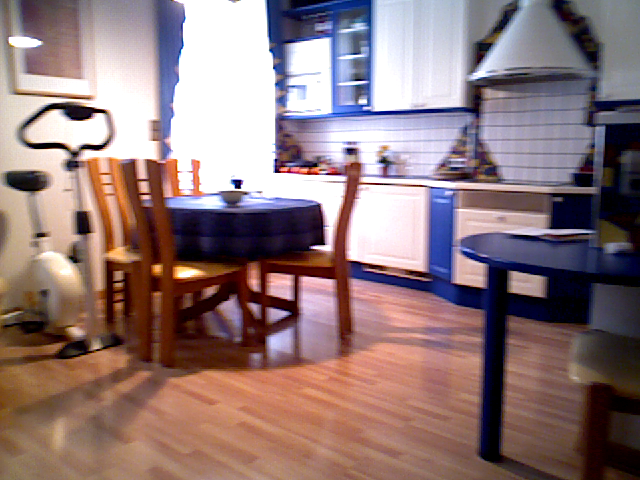
\includegraphics[width=0.7\textwidth,clip]{figures/basic_eval/max_rot_img.png} 
  \caption[Example RGB-image]{An example RGB-image: At the maximum rotational velocity the motion blur is already high. The limited dynamic range is also visible in this image. }
  \label{RotMax}
\end{figure}

\subsubsection{Point clouds}

The quality of the point cloud is good, but obviously not as accurate as the laser scan. The distance range given in the specifications of the RGBD-camera from 0.8\,m to 3.5\,m is very pessimistic. Tests showed a minimum detectable distance of 0.55\,m and a maximum distance much higher than the 3.5\,m. 

\subsection{Computer vision}

\subsubsection{Room type classification}



\subsubsection{Object detection}

\subsubsection{Doorway detection}

The doorway detection works very well, with no wrong detections and no passing of undetected doorways during the test runs. The only problem is the small field of view of the upward looking RGBD-camera. Therefore doorways are only detected if the robot is near the doorway and facing towards the doorway. This means that a doorway may not be detected while driving by.

\subsection{Navigation}

The navigation causes a lot of problems in this work. The main problem is the high payload, which puts too much weight on the passive wheels. This results in less grip on the active wheels. As a result the robot has problems to turn, especially on slippery or uneven ground. In some cases the robot is even unable to turn at all without some help. When executing in-place rotations the robot might drift forwards or backwards. The biggest problem is that the robot has problems to drive curves as planned. The slipping caused the robot to drive curves too wide, which in further consequence lead the robot to get stuck because it got too near to an obstacle. The recovery behaviors may be successful, but sometimes the robot needs help to unstuck. This problem was somewhat solved by increasing all rotational velocities manually before sending them to the Turtlebot. 

\subsection{System Stability}